\graphicspath{{6conics/asy/}}

\section{Conic Sections}

In this section we consider the traditional conic sections and relate their basic properties to modern equations.

\begin{defn}{}{}
A (non-degenerate) \emph{conic section} is the intersection of a \emph{right circular cone}\footnotemark with a plane not passing through the vertex.\smallbreak
Depending on the orientation of this plane, we obtain one of the three standard types of conic section.
\begin{description}
	\item[\normalfont Parabola:] The plane intersects in a single curve either on the upper or lower half of the cone. Equivalently, the plane is parallel to one of the lines defining the cone.
	\item[\normalfont Ellipse:] The intersection is a single closed curve.
	\item[\normalfont Hyperbola:] The intersection comprises two curves, one each on the upper and lower halves of the cone. 
\end{description}
\end{defn}
\begin{center}
\begin{tabular}{c@{\qquad\qquad}c@{\qquad}c}
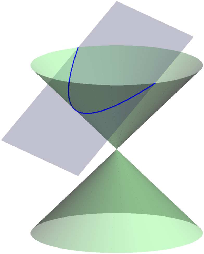
\includegraphics[scale=1.1]{conicparabola_0}
&
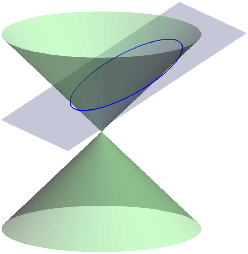
\includegraphics[scale=1.1]{conicellipse_0}
&
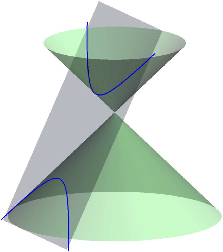
\includegraphics[scale=1.1]{conichyperbola_0}
\\
\href{http://www.math.uci.edu/~ndonalds/math8/conicparabola2.html}{Parabola}
&
\href{http://www.math.uci.edu/~ndonalds/math8/conicellipse2.html}{Ellipse}\phantom{bobob}
&
\href{http://www.math.uci.edu/~ndonalds/math8/conichyperbola2.html}{Hyperbola}
\end{tabular}
\end{center}


\footnotetext{A \emph{cone} is a surface obtained by joining all points on a curve with a fixed point, the \emph{vertex.} A right circular cone is when this curve may be chosen to be a \emph{circle} such that the line from its center to the vertex (the \emph{axis}) is perpendicular (\emph{right angles}) to the circle.}


\begin{tcolorbox}[exercisestyle,title={Exercise}\quad]
Get a piece of paper, make a cone and \emph{draw} some sections!
\end{tcolorbox}

The conic section definitions are hard to work with because they are three dimensional. We instead make alternative definitions as curves in the plane.


\begin{defn}[lower separated=false, sidebyside, sidebyside align=top seam, sidebyside gap=0pt, righthand width=0.35\linewidth]{}{}
Let $d$ be a line in the plane, and $F$ a point not on that line. The \emph{\textcolor{Green}{parabola}} with \emph{directrix} $d$ and \emph{focus} $F$ is the set of points $P$ equidistant from both.\smallbreak
In the language of the picture, $\nm{FP}=\nm{PQ}$.
\tcblower
\flushright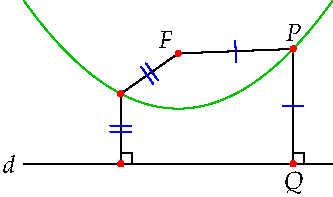
\includegraphics{parabola1}
\end{defn}

The definition is strictly \emph{synthetic} since equidistant really means that the line segments $\cl{FP}$ and $\cl{PQ}$ are \emph{congruent.} To interpret this \emph{analytically} we choose axes and co-ordinates.

\begin{minipage}[t]{0.6\linewidth}\vspace{0pt}
Without loss of generality, choose the origin to lie on the parabola halfway between the focus and directrix and orient things such that the focus lies on the $y$-axis. Otherwise said, for some $a$, the focus has co-ordinates $(0,a)$ and the directrix has equation $y=-a$.\smallbreak
Now we follow the definition: if $P=(x,y)$ is a point on the parabola, then $Q=(x,-a)$, whence
  \begin{align*}
  \nm{FP}=\nm{PQ}&\iff \nm{FP}^2=\nm{PQ}^2\\
  &\iff x^2+(y-a)^2=(y+a)^2
  \end{align*}
\end{minipage}\begin{minipage}[t]{0.4\linewidth}\vspace{0pt}
\flushright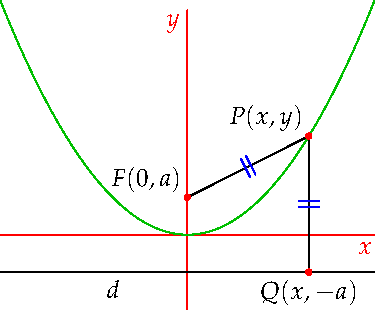
\includegraphics{parabola4}
\end{minipage}


If we multiply out and simplify, we recover a familiar equation:

\begin{thm}{}{}
Given a parabola, there exist rectangular co-ordinates/axes with respect to which the parabola has equation $x^2=4ay$ for some $a>0$. This is the \emph{canonical form} of the parabola.
\end{thm}

Of course parabolas are often not presented to us in canonical co-ordinates.

\begin{example}{}{parabola}
Find the focus and directrix of the parabola with equation $y=x^2-6x+7$.\smallbreak
Complete the square!
\[y=x^2-6x+7=(x-3)^2-2\]
\begin{minipage}[t]{0.65\linewidth}\vspace{-5pt}
With respect to new co-ordinates $X=x-3$ and $Y=y+2$ we obtain the canonical form
\[X^2=Y=4aY\iff a=\frac 14\]
The focus has co-ordinates $(X,Y)=(0,\frac 14)$ and the directrix is $Y=-\frac 14$. Translating back to our original co-ordinates we obtain
\[F=(3,-\tfrac 74),\qquad \text{Directrix}: y=-\frac 94\]
\end{minipage}
\begin{minipage}[t]{0.35\linewidth}\vspace{-10pt}
\flushright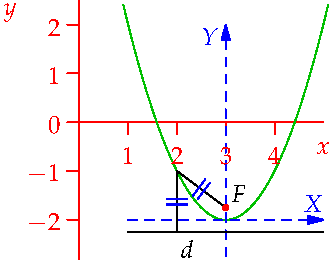
\includegraphics{parabola3}
\end{minipage}
\end{example}

Canonical co-ordinates can also be rotated relative to given axes, but this would take us too far afield.

\boldinline{Relation to the cone}

The simplest way to see this is to suppose that the cone is centered on the $z$-axis and has equation $z^2=x^2+y^2$: the cross-section a distance 1 up the $z$-axis is a circle of radius 1. The point $(x,y,z)=(0,1,1)$ certainly lies on the cone: any plane parallel to this has equation $z=y+k$ for some constant $k$. Now substitute
\[\begin{cases}
z^2=x^2+y^2\\
z=y+k
\end{cases} \implies (y+k)^2=x^2+y^2\implies x^2=2ky+k^2\]
which is the equation\footnote{Strictly this is the equation of the \emph{projection} of the parabola onto the $xy$-plane. We should really pull out a factor of $\sqrt{2}$ from $y$ to compensate for the slope of the intersecting plane.} of a parabola!

\begin{tcolorbox}[exercisestyle,title={Why call it the \emph{focus}?}\quad]
A \emph{parabolic mirror} is a reflective surface obtained by rotating a parabola around its canonical $y$-axis. Imagine a light source at `vertical infinity,' whose rays therefore arrive parallel to the $y$-axis. The parabolic mirror will focus these rays onto the focus of the original parabola! This is the reason that satellite dishes are parabolic, with the receiver placed at their focus.\smallbreak

The argument requires only a little triangle geometry.
 
	\begin{minipage}[t]{0.6\linewidth}\vspace{0pt}
	  Let $P$ lie on the parabola, $Q$ its nearest point on the directrix and bisect angle $\angle FPQ$ with the line $\ell$. Let $R\neq P$ be any other point on $\ell$.
	  \begin{enumerate}
	    \item Why do we have $\nm{FR}=\nm{RQ}$?
	    \item Why is $\nm{RS}<\nm{FR}$?
	    \item Why does this force $\ell$ to be the \emph{tangent line} to the parabola?
	    \item Why can we conclude that the vertical ray hitting the mirror at $P$ is reflected towards $F$?
	  \end{enumerate}
	\end{minipage}\begin{minipage}[t]{0.4\linewidth}\vspace{0pt}
	\flushright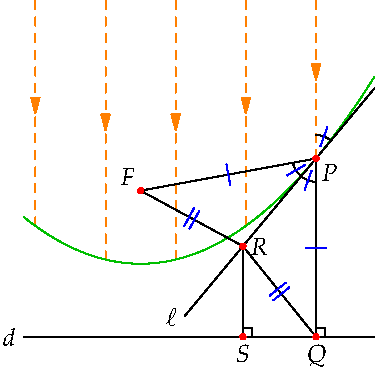
\includegraphics{parabola2}
	\end{minipage}
\end{tcolorbox}
If you want a hard life, try arguing using equations and analytic geometry :)\bigbreak

Now we turn to the planar definition of an ellipse.

\begin{defn}[lower separated=false, sidebyside, sidebyside align=top seam, sidebyside gap=0pt, righthand width=0.35\linewidth]{}{}
Let $F,G$ be points in the plane and $a>\frac 12\nm{FG}$ a positive constant. The set of points $P$ such that
\[\nm{FP}+\nm{GP}=2a\]
is an \emph{ellipse} with \emph{foci} $F,G$ and \emph{semi-major axis} $a$. If $F=G$, the ellipse is a circle with radius $a$.
\tcblower
\flushright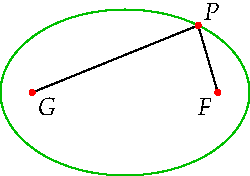
\includegraphics{ellipse1}
\end{defn}

\begin{exercises}{}{}
\hangindent\leftmargini
\textup{1. } To put this in canonical form, suppose the foci lie on the $x$-axis with the origin at their midpoint: $F=(c,0)$ and $G=(-c,0)$ for some $c$. Start by squaring
\begin{align*}
(x-c)^2+y^2&=\nm{FP}^2=(2a-\nm{GP})^2=\left(2a-\sqrt{(x+c)^2+y^2}\right)^2\\
&=4a^2+(x+c)^2+y^2-4a\sqrt{(x+c)^2+y^2}
\end{align*}

\begin{enumerate}\setcounter{enumi}{1}
  \begin{minipage}[t]{0.6\linewidth}\vspace{-10pt}
\item[]then rearrange to place the remaining square-root on one side before squaring to eliminate. After simplifying, you should obtain the familiar form
\[\frac{x^2}{a^2}+\frac{y^2}{b^2}=1\quad\text{where}\quad b^2=a^2-c^2\]
The value $b$ is called the \emph{semi-minor} axis. Hopefully the meaning of these terms is clear from the picture.
\end{minipage}\begin{minipage}[t]{0.4\linewidth}\vspace{-30pt}
\flushright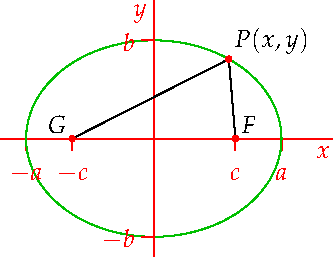
\includegraphics{ellipse2}
\end{minipage}
	
	\goodbreak

  \item Similarly to Example \ref{ex:parabola}, complete the square for both $x$ and $y$ to show that the equation
\[9x^2+4y^2-36x-8y+4=0\]
represents an ellipse. Sketch it and find the co-ordinates of its foci.


  \begin{minipage}[t]{0.6\linewidth}\vspace{0pt}
	\item A reflection principle also applies to the ellipse. It is a little different from the parabola since we now have two foci.
	\begin{itemize}
	  \item Extend $\cl{GP}$ to $Q$ such that $\nm{PQ}=\nm{PF}$.
	  \item Bisect $\angle FPQ$ by the line $\ell$.
	  \item If $R$ is any other point on $\ell$, explain why
	  \[\nm{FR}+\nm{GR}>2a\]
	  and thus why $R$ lies \emph{outside} the ellipse.
	  \item Hence explain why a light source placed at one focus will have its rays reflected by an elliptical mirror onto the other focus.
	\end{itemize}
\end{minipage}\begin{minipage}[t]{0.4\linewidth}\vspace{0pt}
\flushright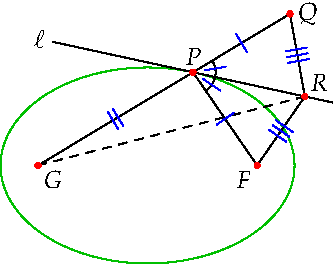
\includegraphics{ellipse3}\\
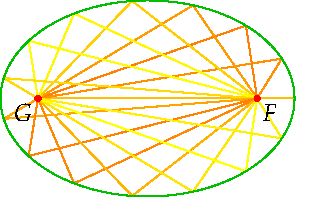
\includegraphics{ellipse4}
\end{minipage}
\end{enumerate}
\end{exercises}


\begin{defn}[lower separated=false, sidebyside, sidebyside align=top seam, sidebyside gap=0pt, righthand width=0.35\linewidth]{}{}
Let $F,G$ be points in the plane and $a<\frac 12\nm{FG}$ a positive constant. The set of points $P$ such that
\[\nm{FP}-\nm{GP}=\pm 2a\]
is a \emph{hyperbola} with \emph{foci} $F,G$.
\tcblower
\flushright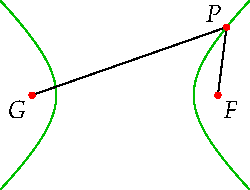
\includegraphics{hyperbola1}
\end{defn}

\begin{tcolorbox}[exercisestyle,lower separated=false, sidebyside, sidebyside align=top seam, sidebyside gap=0pt, righthand width=0.35\linewidth]{}{}
\hangindent\leftmargini
\textup{1. } Exactly as above, verify that by choosing $F=(c,0)$ and $G=(-c,0)$, a hyperbola has equation
\[\frac{x^2}{a^2}-\frac{y^2}{b^2}=1\quad\text{where}\quad b^2=c^2-a^2\]
\begin{enumerate}\setcounter{enumi}{1}
  \item As $x\to\infty$ show that the hyperbola approaches its \emph{asymptotes} $y=\pm \frac bax$.
  \item (Challenge!)\quad Verify the `reflection' principle for hyperbolæ: if a light source is placed at a focus, then the reflected rays will appear to have emanated from the \emph{other} focus.
\end{enumerate}
\tcblower
\flushright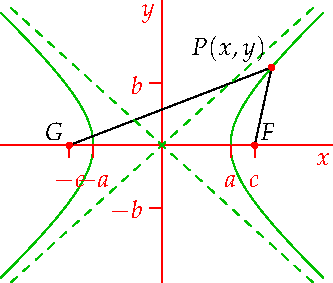
\includegraphics{hyperbola2}
\end{tcolorbox}


\boldsubsubsection{Eccentricity}

The obvious difference between our descriptions of the ellipse/hyperbola versus the parabola is the \emph{directrix.}

\begin{thm}{}{}
Let $F$ be a point (the \emph{focus}) not on a line $d$ (the \emph{directrix}) and choose a number $e>0$ (the \emph{eccentricity}). Consider the set of points $P$ satisfying
\[\nm{PF}=e\nm{PQ}\]
where $Q$ is the nearest point to $P$ on the directrix.
\begin{enumerate}
  \item Depending on the value of $e$ we obtain one of the three conic sections. For the ellipse and the hyperbola this construction only produces half of the conic; there are in fact \emph{two} directrices.
	\begin{center}
		\begin{tabular}{c@{\qquad}c@{\qquad\qquad}c}
		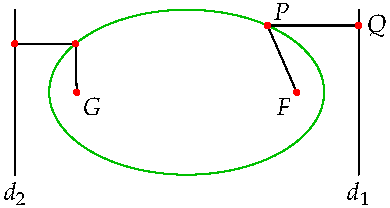
\includegraphics{eccentricity2}
		&
		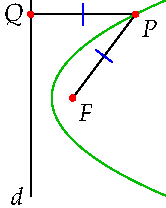
\includegraphics{eccentricity}
		&
		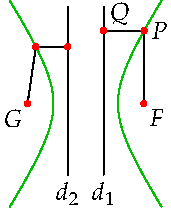
\includegraphics{eccentricity3}
		\\
		Ellipse $e<1$&Parabola $e=1$&Hyperbola $e>1$
		\end{tabular}
	\end{center}
	\item For the ellipse and hyperbola $e=\frac ca$, where $c=\frac 12\nm{FG}$.
	%\item If a plane intersects a right circular cone $z^2=x^2+y^2$ at an angle of $\alpha$ to the horizontal (i.e. $z=\tan\alpha y+k$), then $e=\sqrt 2\cos\alpha$.
\end{enumerate}
\end{thm}

By convention, a circle is considered to have eccentricity $e=0$, even though the above doesn't apply. We could imagine obtaining a circle of radius $a$ by taking the limit $e\to 0^+$ (i.e.\ $c\to 0^+$). In such a limit, the point $Q$ on the directrix must go to infinity: circles therefore do not have directrices!

\begin{example}{}{}
The canonical form ellipse $\frac{x^2}{25}+\frac{y^2}{16}=1$ has $a=5,b=4$ and $c=\sqrt{a^2-b^2}=3$. Its eccentricity is therefore $e=\frac ca=\frac 35$. Since its foci have co-ordinates $(\pm\frac 35,0)$, its right directrix must be a vertical line which intersects the $x$-axis when
\[e(x-a)=(a-c)\implies x=a+\frac{a-c}e=5+\frac{10}3=\frac{25}3\]
\end{example}

\begin{exercises}{}{}
\hangindent\leftmargini
\textup{1. } Find the foci and directrices of the hyperbola $\frac{x^2}{16}-\frac{y^2}{9}=1$. Sketch the curve.
\begin{enumerate}\setcounter{enumi}{1}
  \item Verify some of the theorem. 
\end{enumerate}
\end{exercises}

After refreshing some trigonometry, we'll return to conics. In particular we'll see how they may be parametrized, and how the eccentricity relates to the cone/plane combination which created the conic in the first place!


%Trig functions after and use them to parametrise conics

% Do polar co-ords and complex numbers to normalize?

% \begin{example}{}{}
% Real world data is unlikely to be so compliant. If we have the 
% \end{example}

% AFTER MIDTERM: conic sections. Parabola, ellipse and hyperbola old-school style. reflections, etc. Mirror. Planet orbits? Gauss and regression/normal distribution.

% Exponentials are an invaluable 
% 
% If we think that we have data which appears to be growing 

% \boldsubsubsection{Periodic Functions and Trigonometry}
% 
% \begin{defn}{}{}
% A function $f$ is \emph{periodic} with period $T$ if, for all $x\in\dom f$,
% \[f(x+T)=f(x)\]
% \end{defn}
% 
% \begin{example}{}{}
% The \emph{floor} $\lfloor x\rfloor$ of a real number $x$ is the largest integer less than or equal to $x$. For example
% \[\lfloor 2.5\rfloor =2,\qquad \lfloor \pi\rfloor=3,\qquad\lfloor -\sqrt 2\rfloor=-2,\qquad \lfloor -11\rfloor=-11\]
% Since $\lfloor x+1\rfloor=1+\lfloor x\rfloor$ for any $x$, the \emph{fractional part} function $f(x)=x-\lfloor x\rfloor$ is periodic with period 1, since
% \[f(x+1)=f(x)\]
% \end{example}
% 
% \begin{defn}{Trig functions}{}
% The basic trig functions are periodic: measure the angle counter-clockwise from the positive real axis.
% \end{defn}
% 